% pres_solar_prod.tex

\documentclass{beamer}
\usepackage{url}
\usepackage{amsmath}
\usepackage{esdiff} %for writing partial derivatives
\usetheme{default}

\title{Lease or Buy?}
\subtitle{Quality differences and asymmetric information in California solar panels}
\author[J. Mauritzen]{Johannes Mauritzen \\ NHH Norwegian School of Economics}
\institute[NHH]{
 % Department of Business and Management Science\\
 % NHH Norwegian School of Economics\\[1ex]
  \texttt{jmaurit@gmail.com}
}

\date{\today}

\begin{document}

%--- the titlepage frame -------------------------%
\begin{frame}[plain]
  \titlepage
\end{frame}


%--- the presentation begins here ----------------%

\begin{frame}[plain]
	\begin{itemize}
	\item[] What's behind the surge in the California rooftop solar market? The role of Chinese panels, uncertainty and new business models.
	\item[] \url{jmaurit.github.io\#solar_lemons}
	\end{itemize}
\end{frame}

\begin{frame}[plain]
	\begin{figure}
	\includegraphics[width=1\textwidth]{figures/cost_over_time.png}
	%\caption{After about 2010, prices for solar systems fell dramatically and installations nearly tripled.}
	%\label{cost_over_time}	
	\end{figure}
\end{frame}

\begin{frame}[plain]
	\begin{figure}
		\includegraphics[width=1\textwidth]{figures/top_contractors_plot.png}
		 %\caption{Marked concentration increased markedly over the period studied.  How did Solar City and Verengo gain market share?}
		%\label{top_contractors}	
	\end{figure}	
\end{frame}

\begin{frame}[plain]
	\begin{figure}
		\includegraphics[width=.8\textwidth]{figures/panel_makers_scty.png}
		 %\caption{The top panel makers used by the leading solar system contractor, Solar City. 2011 the company shifted to using panels from relatively unknown chinese manufacturers.}
		%\label{panel_makers_scty}	
	\end{figure}
\end{frame}

\begin{frame}[plain]
	\begin{figure}
		\includegraphics[width=1\textwidth]{figures/scty_china_lease.png}
		 %\caption{Contractors that gained market share, notably Solar City, did so not only by switching to cheaper Chinese panels but also by moving to a leasing model of sales.}
		%\label{cont_market_share}	
	\end{figure}
\end{frame}

\begin{frame}[plain]
	\begin{figure}
	\includegraphics[width=1\textwidth]{figures/chinese_panel_switch.png}
	%\caption{It seems a switch to cheaper Chinese panels can at least partly explain the increased market share of Solar City and Verengo.  But why did so few other contractors adopt Chinese panels?}
	%\label{chinese_panel_switch}	
	\end{figure}	
\end{frame}

\begin{frame}[plain]
	\begin{figure}
		\includegraphics[width=1\textwidth]{figures/solar_panel_review.png}
		%\caption{Websites are available providing reviews of various solar panels, however information is not available on new Chinese manufacturers that have not been on the market.}
		%\label{solar_panel_review}	
	\end{figure}	
\end{frame}

\begin{frame}[plain]
	\begin{figure}
		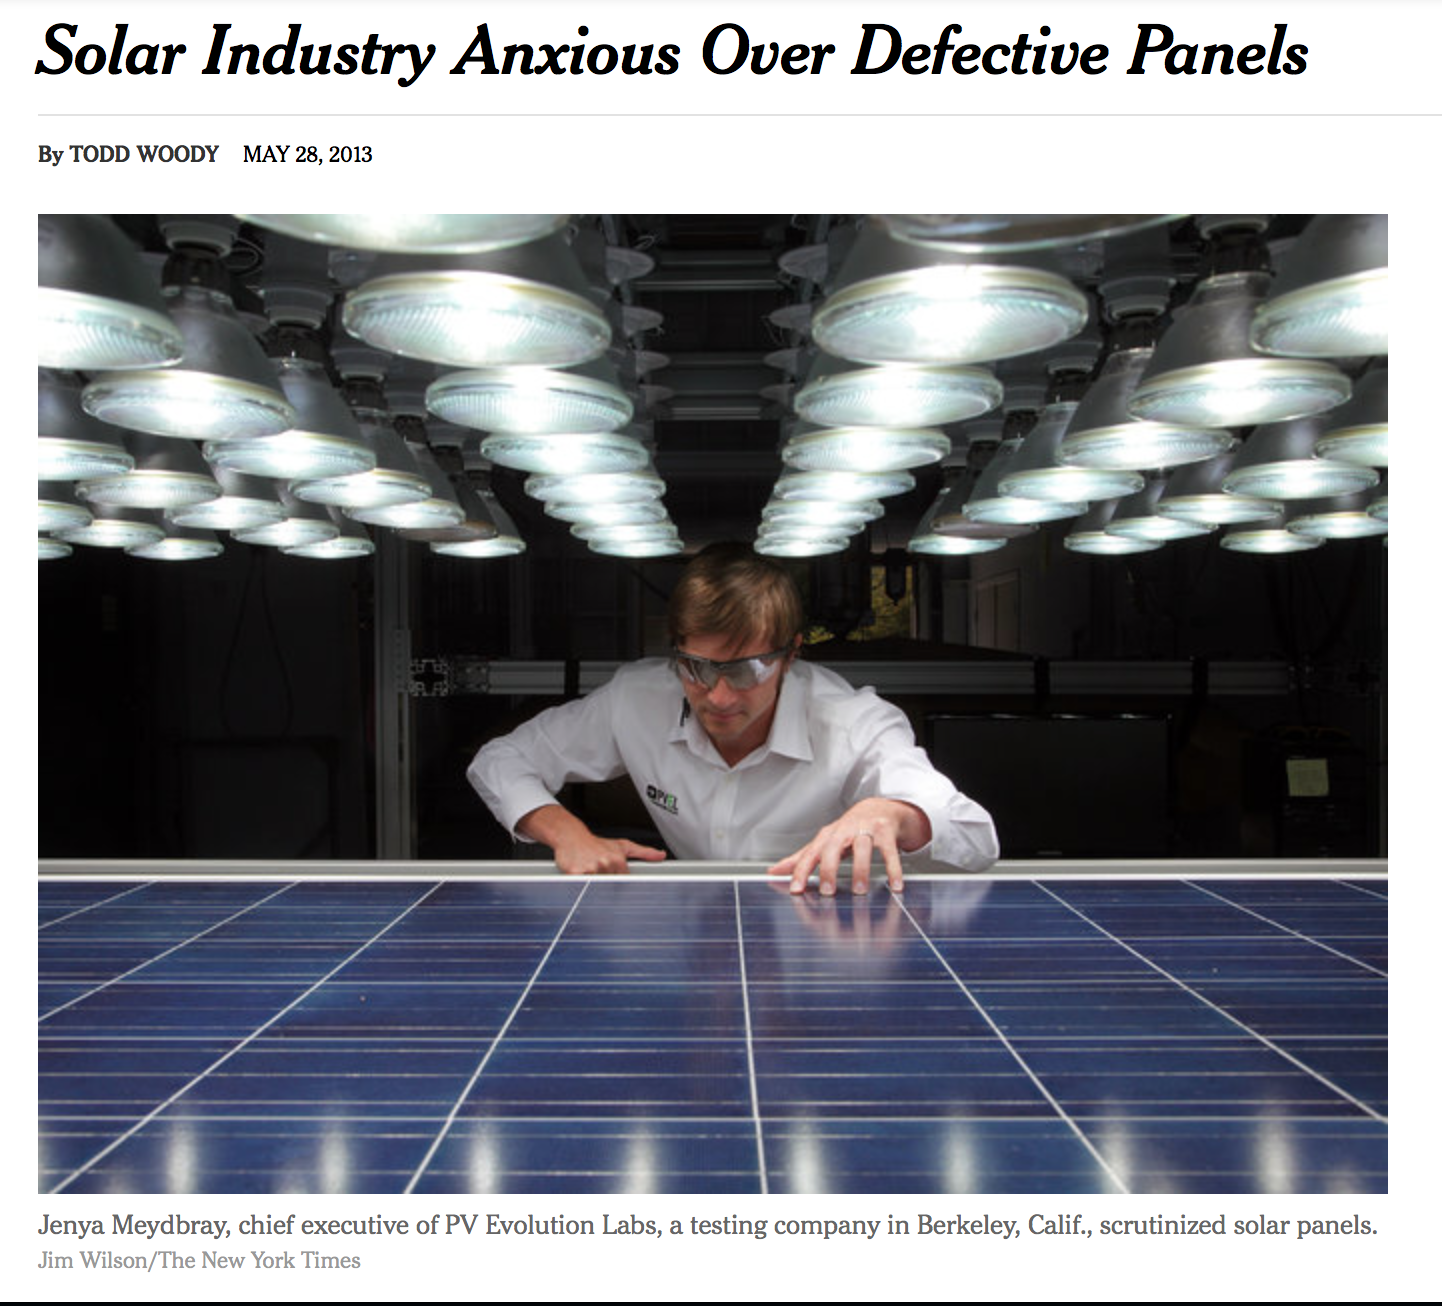
\includegraphics[width=.8\textwidth]{figures/solar_quality_nyt.png}
		%\caption{Websites are available providing reviews of various solar panels, however information is not available on new Chinese manufacturers that have not been on the market.}
		%\label{solar_panel_review}	
	\end{figure}
\end{frame}

\begin{frame}[plain]
	\begin{equation}
	\begin{split}
		lease_i = & invlogit(\alpha + \beta timeYears_i + nationality_i +\\ 
		& \sigma timeYears_i*nationality_i + \epsilon)
		%\label{equation:lease_model}
	\end{split}
	\end{equation}	
\end{frame}


\begin{frame}[plain]
	\begin{figure}
		\includegraphics[width=1\textwidth]{figures/logit_plot.png}
		%\caption{Systems with Chinese panels, mostly absent from the market before 2010, were substantially more likely to be used in leased systems than panels from more established Japanese and German manufacturers.}
		%\label{logit_plot}
	\end{figure}	
\end{frame}



\begin{frame}[plain]
	\begin{equation}
		log(costPerKw_i) = \alpha + \gamma china_i + \tau lease_i + \beta timeYears_i + \sigma inter_i + \epsilon
		%\label{equation:slope1}
	\end{equation}	
\end{frame}



\begin{frame}[plain]
	\begin{figure}
		\includegraphics[width=1\textwidth]{figures/cost_plot.png}
		 %\caption{Systems with Chinese panels are substantially cheaper, but only became widely popular after 2011.}
		%\label{cost_plot}
	\end{figure}
\end{frame}

\begin{frame}
	Quality and Asymmetric Info in Solar Panels
	\begin{itemize}
	\item ``Experience goods''
	\item Hard to ascertain quality, even after the fact
	\item One shot vs. repeat buyers
	\item Warranties may not provide much assurance
	\end{itemize}	
\end{frame}

\begin{frame}
	\begin{figure}
		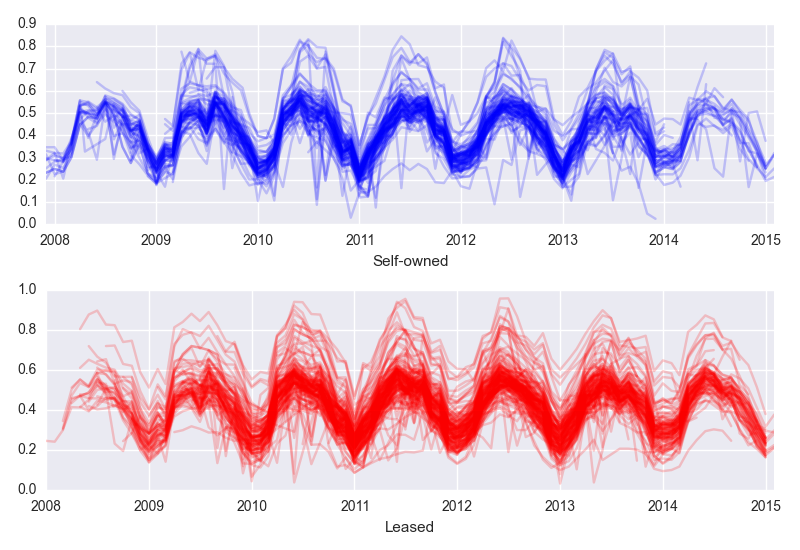
\includegraphics[width=1\textwidth]{tot_production.png}
		% \caption{}
		%\label{tot_production}
	\end{figure}
\end{frame}

\begin{frame}
	\begin{figure}
		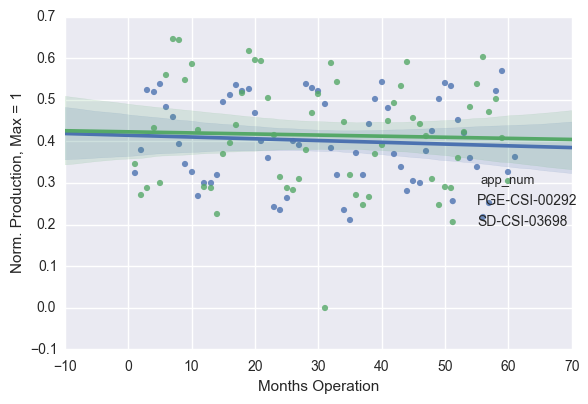
\includegraphics[width=1\textwidth]{example_prod.png}
		%\caption{}
		\label{example_prod}
	\end{figure}
\end{frame}

\begin{frame}
	Hierarchical Bayesian Model
	\begin{itemize}
	\item Natural modeling of structure of data
	\item Natural interpretation of uncertainty
	\item Flexibility of simulation methods
	\end{itemize}	
\end{frame}

\begin{frame}
	\begin{figure}
		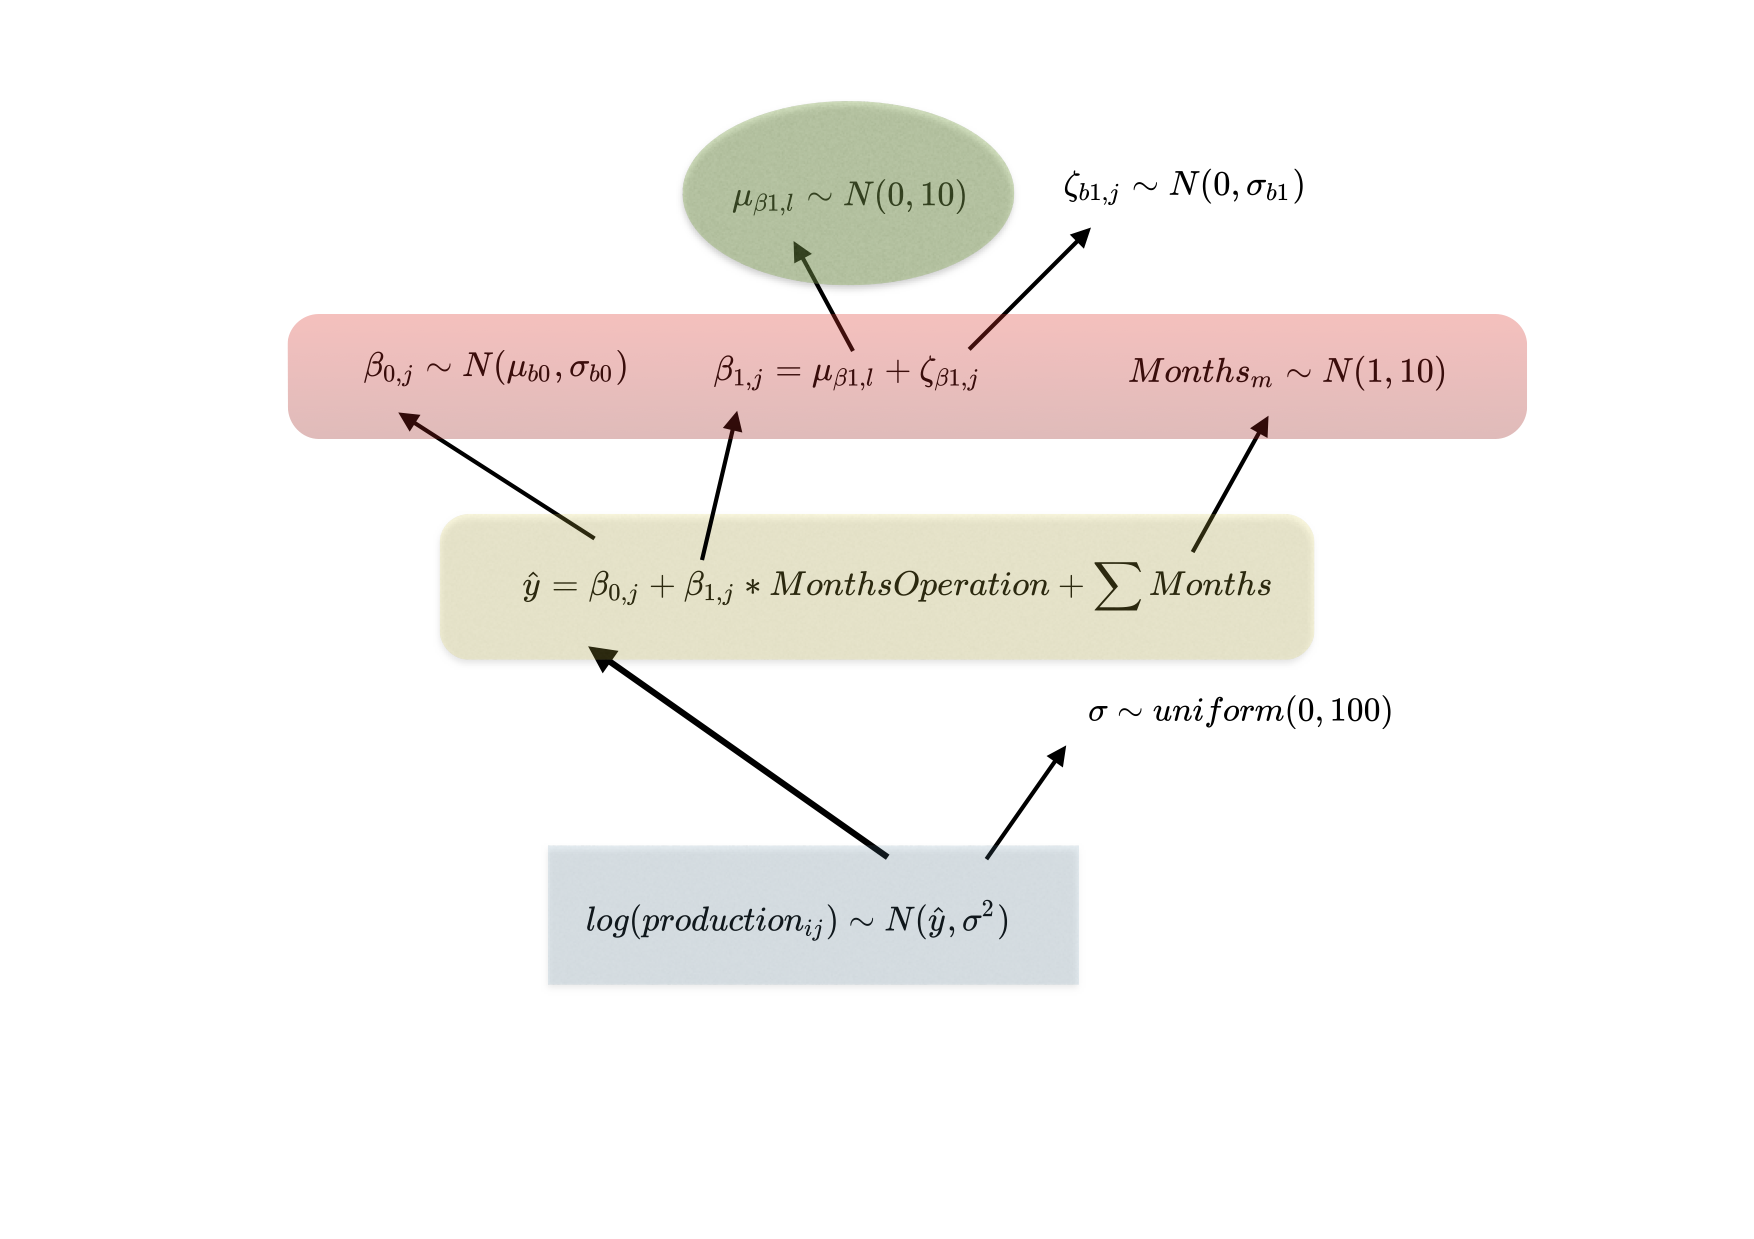
\includegraphics[width=1\textwidth]{solar_prod_bayes_diag.png}		
		%\label{example_prod}
	\end{figure}
\end{frame}

\begin{frame}
	\begin{figure}
		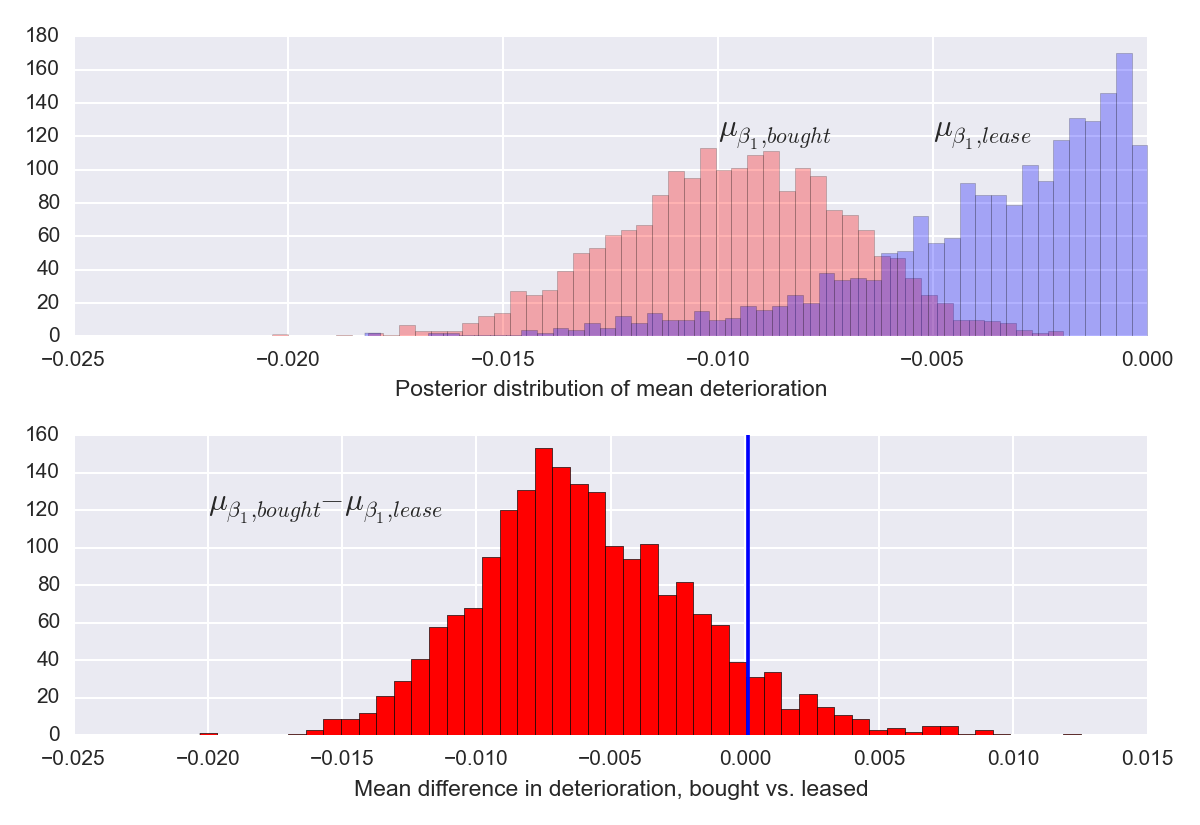
\includegraphics[width=.8\textwidth]{figures/post_mu_b1.png}
		
		\label{post_mu_b1}
	\end{figure}
\end{frame}

\begin{frame}
	\begin{figure}
		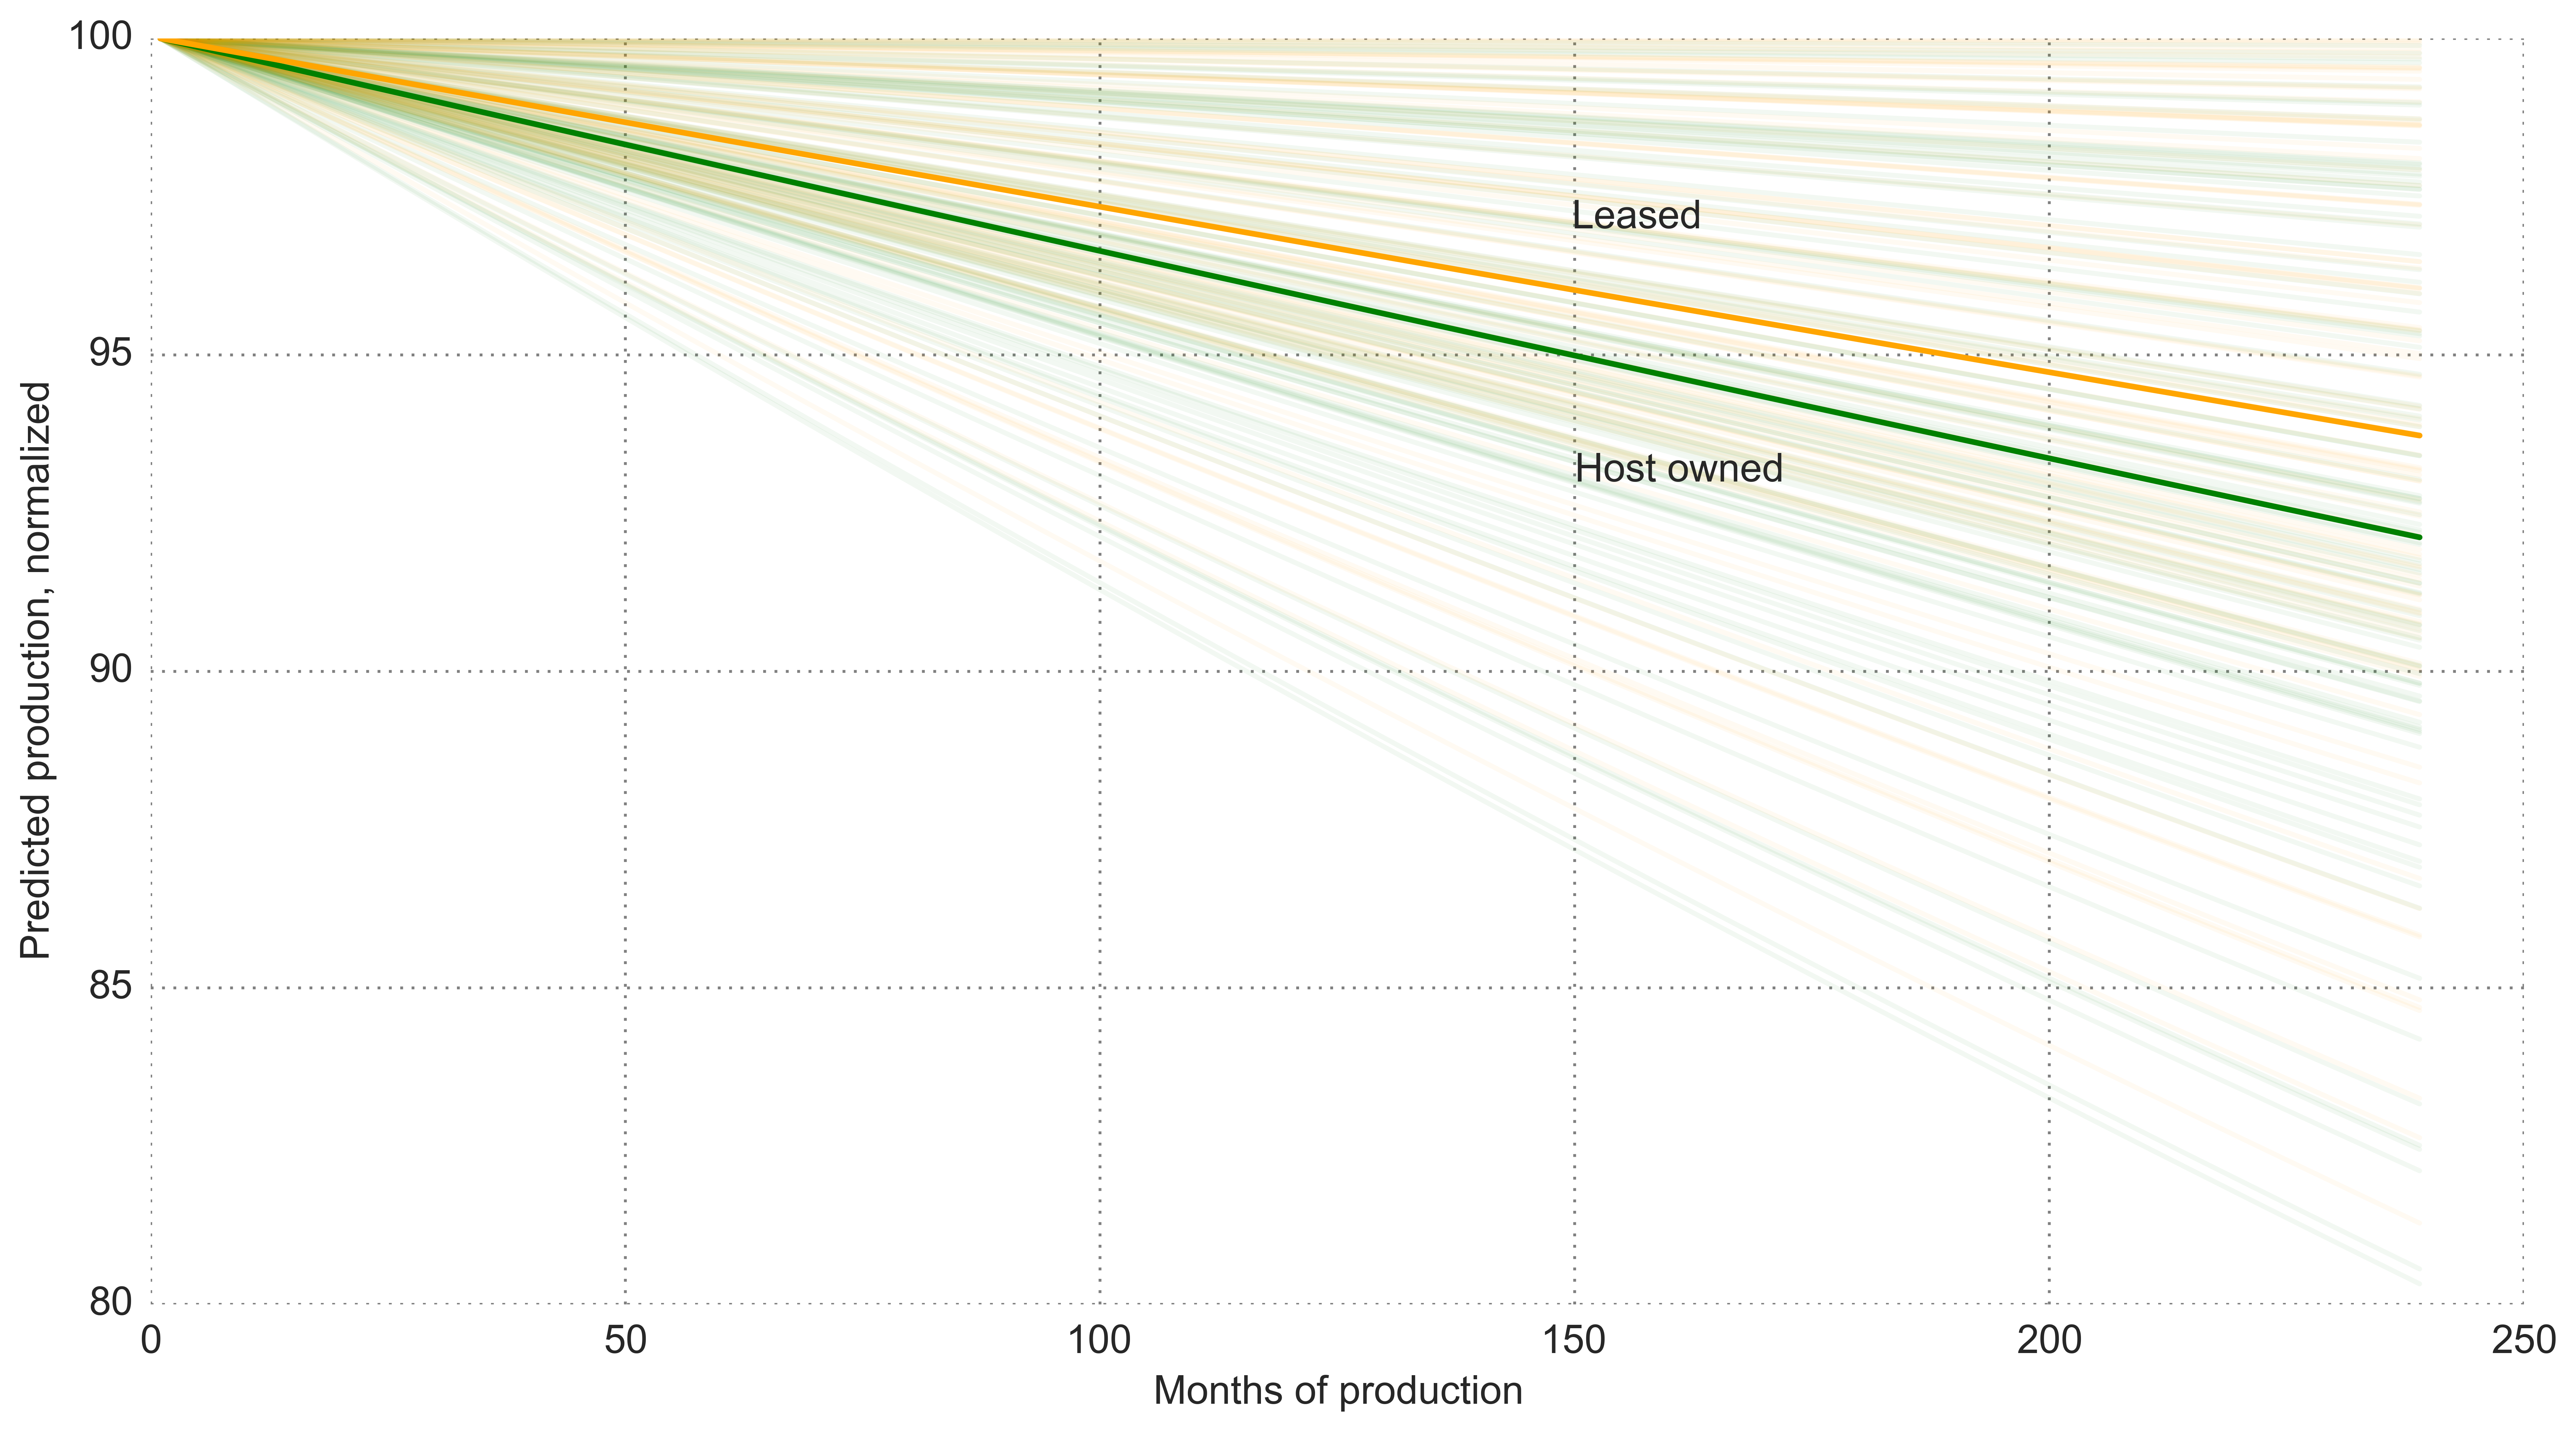
\includegraphics[width=.8\textwidth]{figures/predicted_deg.png}
		\label{predicted_deg}
	\end{figure}
\end{frame}

\begin{frame}[plain]
\textbf{Main Points:}
	\begin{itemize}
	\item Cheaper Chinese panels AND the introduction of a leasing business model are directly linked to the surge in solar panel installations. 
	\end{itemize}
\end{frame}

\begin{frame}[plain]
\textbf{Main Points:}
	\begin{itemize}
	\item Cheaper Chinese panels AND the introduction of a leasing business model are directly linked to the surge in solar panel installations. 
	\item Leasing could be an effective way of getting over issues of asymmetric information on quality. 
	\end{itemize}
\end{frame}

\begin{frame}[plain]
\textbf{Main Points:}
	\begin{itemize}
	\item Cheaper Chinese panels AND the introduction of a leasing business model are directly linked to the surge in solar panel installations. 
	\item Leasing could be an effective way of getting over issues of asymmetric information on quality. 
	\item Leased systems tend to have lower degradation over time than those sold outright, consistent with the economic theory on the subject.
	\end{itemize}
\end{frame}

\begin{frame}[plain]
	\begin{itemize}
	\item[] \textbf{Main Lesson for Managers:} Managers need to address uncertainty about quality when selling energy investment goods to consumers and small businesses with limited financial and engineering resources.
	\end{itemize}
\end{frame}

\begin{frame}[plain]
	\begin{itemize}
	\item[] \textbf{Policy Implications:} Flexible support schemes are important for allowing business model innovations and increased investment in renewable energy.
	\end{itemize}
\end{frame}

\begin{frame}[plain]
	\begin{figure}
		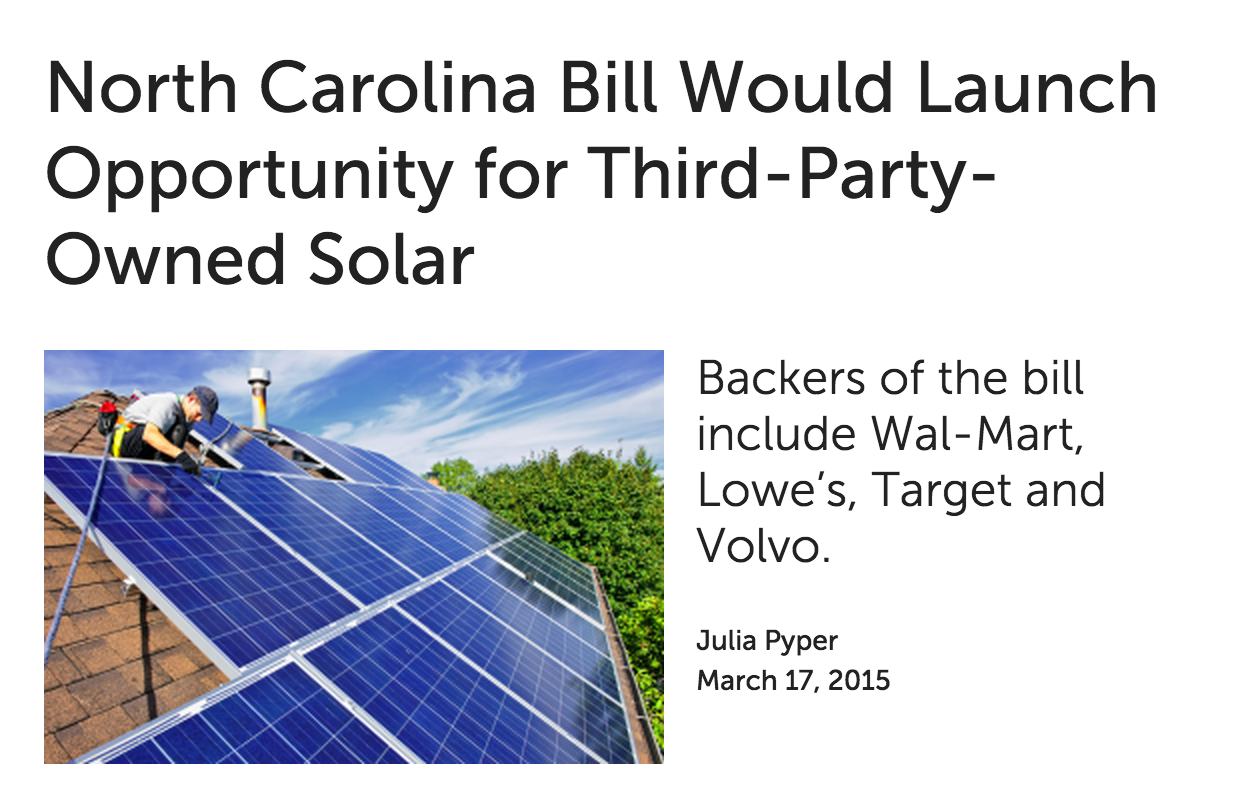
\includegraphics[width=1\textwidth]{figures/Northcarolina_3rd_party_law.png}
	
	\end{figure}
\end{frame}


\begin{frame}[plain]
	\begin{itemize}
	\item[] \textbf{Indirect Policy Implication:} Simultaneously subsidizing an investment and adding import duties appear to be contradictory.  
	\end{itemize}
\end{frame}

\end{document}

